\lab{Algorithms}{Canonical Transformations and the QR Decomposition}{Canonical Transformations and the QR Decomposition}
\label{Ch:Canonical Transformations}

\objective{Use orthogonal transformations to perform QR decomposition.}

\section*{Orthogonal transformations}
Recall that a matrix $Q$ is \emph{unitary} if $Q^* Q = I$ or for real matrices, $Q^T Q = I$ (since the conjugate of a real number is itself). We like unitary transformations because they're very numerically stable. The number $\kappa(A) = \norm{A} \norm{A^{-1}}$ is called the \emph{condition number} of $A$. We'll discuss condition number more in Lab \ref{Ch:Norms and Geometry}; for now, all you need to know is that if $\kappa(A)$ is small, then problems involving $A$ are less susceptible to numerical errors. For induced matrix norms (which include most of the matrix norms we would ever care about),  it holds that $\norm{Q}=1$ when $Q$ is unitary. The inequality $\norm{AB} \leq \norm{A} \norm{B}$ also holds for these norms. It follows that $\kappa(A) = \norm{A} \norm{A^{-1}} \geq \norm{A A^{-1}} = \norm{I} = 1$. Note that if $Q$ is unitary, $Q^{-1} = Q^*$ and $Q^*$ is also unitary, so $\kappa(Q) = \norm{Q} \norm{Q^*} = 1$. This means that orthogonal matrices have the smallest possible condition number, which is great!

Any unitary matrix $Q$ can be described as a reflection, a rotation, or some combination of the two. If $det(Q) = 1$, then $Q$ is a rotation; if $det(Q) = -1$, then $Q$  is the composition of a reflection and a rotation.  Let's explore these two types of unitary transformations and some of their applications. We will focus on the real case to simplify matters.

\section*{Householder reflections}
A Householder reflection is a linear transformation $P: \mathbb{R}^n \rightarrow \mathbb{R}^n$ that reflects a vector $x$ about a hyperplane. See figure \ref{fig:Householder reflector}. Recall that a hyperplane can be defined by a unit vector $v$ which is orthogonal to the hyperplane. As shown in the figure, $x - \langle v,x \rangle v$ is the projection of $x$ onto the hyperplane defined by $v$. (You should verify this geometrically.) However, to reflect \emph{across} the hyperplane, we must move twice as far; that is, $Px = x - 2\langle v,x \rangle v$. This can be written $Px = x - 2v(v^\ast x)$, so $P$ has matrix representation $P = I - 2vv^\ast$. Note that $P^\ast P = I$; thus $P$ is orthogonal.

\begin{figure}
	\centering
	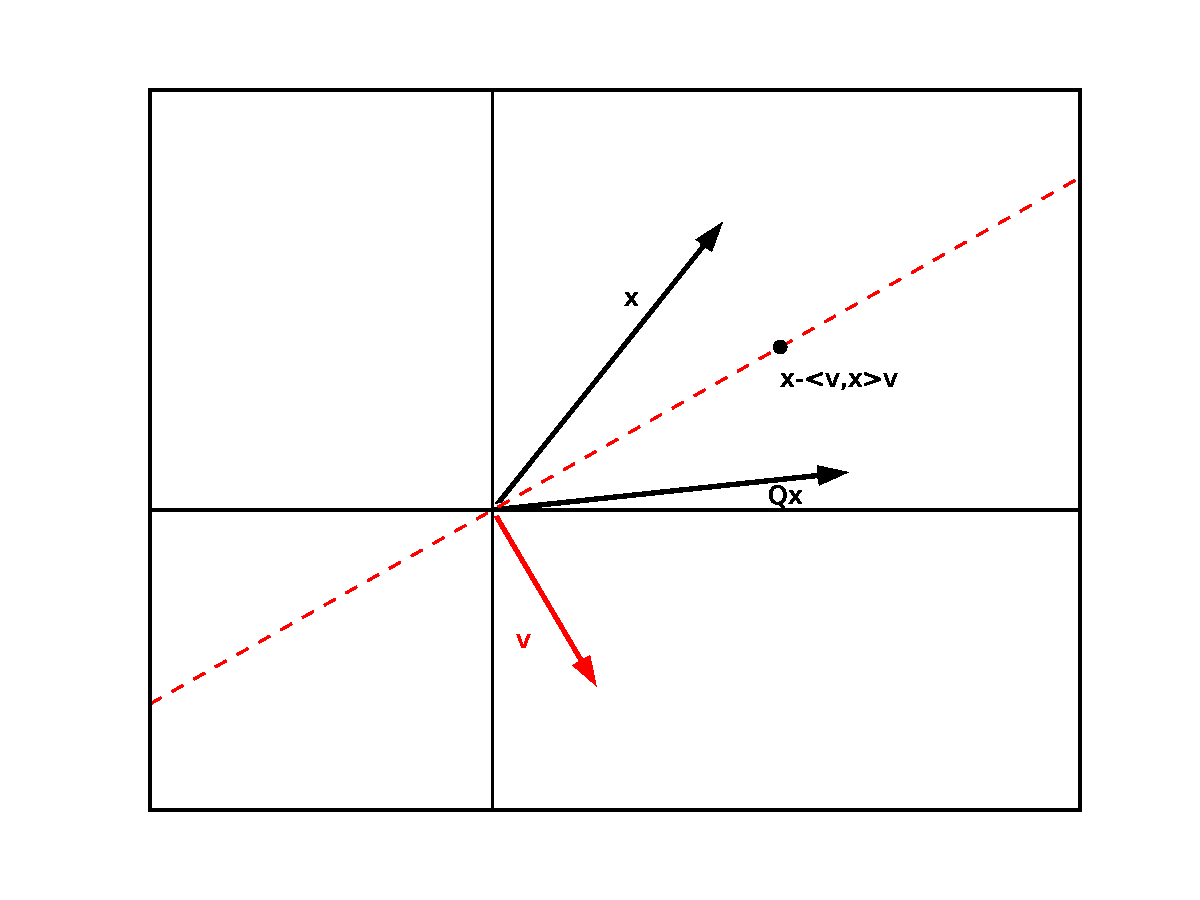
\includegraphics[width= \textwidth]{fig1}
	\caption{Householder reflector}
	\label{fig:Householder reflector}
\end{figure}

\subsection*{Householder triangularization}
Consider the problem of computing the $QR$ decomposition of a matrix $A$. You've already learned the Gram-Schmidt and the Modified Gram-Schmidt algorithms for this problem. The $QR$ decomposition can also be computed using Householder triangularization. Gram-Schmidt and Modified Gram-Schmidt \emph{orthogonalize} $A$ by a series of \emph{triangular} transformations. Conversely, the Householder method \emph{triangularizes} $A$ by a series of \emph{orthogonal} transformations.

Let's demonstrate this method on a $4 \times 3$ matrix $A$. First we find a orthogonal transformation $Q_1$ that maps the first column of A into the range of $e_1$.

\def\mc#1{\multicolumn{1}{c|}{#1}}
\begin{equation*}
\begin{pmatrix}
\ast & \ast & \ast \\
\ast & \ast & \ast \\
\ast & \ast & \ast \\
\ast & \ast & \ast 
\end{pmatrix}
\underrightarrow{Q_1}
\begin{pmatrix}

\ast & \ast & \ast & \\ \cline{2-3}
\mc{0} & \ast & \mc{\ast}& \\
\mc{0} & \ast & \mc{\ast} & \\
\mc{0}& \ast & \mc{\ast} & \\ \cline{2-3}
\end{pmatrix}
\end{equation*}
Let $A_2$ be the boxed submatrix of $A$. Now find an orthogonal transformation $Q_2$ that maps the first column of $A_2$ into the range of $e_2$. 

\begin{equation*}
\begin{pmatrix}
\ast & \ast \\
\ast & \ast \\
\ast & \ast 
\end{pmatrix}
\underrightarrow{Q_2}
\begin{pmatrix}
\ast & \ast \\
0 & \ast \\
0 & \ast 
\end{pmatrix}
\end{equation*}
Similarly, $ \begin{pmatrix} \ast \\ \ast \end{pmatrix} \underrightarrow{Q_3} \begin{pmatrix} \ast \\ 0 \end{pmatrix} $. (Technically $Q_2$ and $Q_3$ act on the whole matrix and not just on the submatrices, so that $Q_i: \mathbb{R}^n \rightarrow \mathbb{R}^n$ for all $i$. $Q_2$ leaves the first row alone, and $Q_3$ leaves the first two rows alone.) Then $Q_3 Q_2 Q_1 A =$ 

\begin{equation*}
Q_3 Q_2 Q_1
\begin{pmatrix}
\ast & \ast & \ast \\
\ast & \ast & \ast \\
\ast & \ast & \ast \\
\ast & \ast & \ast \\
\end{pmatrix}
= Q_3 Q_2
\begin{pmatrix}
\ast & \ast & \ast \\
0 & \ast & \ast \\
0 & \ast & \ast \\
0 & \ast & \ast \\
\end{pmatrix}
= Q_3
\begin{pmatrix}
\ast & \ast & \ast \\
0 & \ast & \ast \\
0 & 0 & \ast \\
0 & 0 & \ast \\
\end{pmatrix}
= 
\begin{pmatrix}
\ast & \ast & \ast \\
0 & \ast & \ast \\
0 & 0 & \ast \\
0 & 0 & 0 \\
\end{pmatrix}
\end{equation*}

We've accomplished our goal, which was to triangularize $A$ using orthogonal transformations. But now, how do we find the $Q_i$ that do what we want? Using Householder reflections. (Surprise!)

For example, to find $Q_1$, we choose the right hyperplane to reflect $x$ into the range of $e_1$. It turns out there are two hyperplanes that will work, as shown in figure \ref{fig:two reflectors}. (In the complex case, there are infinitely many such hyperplanes.) Between the two, the one that reflects $x$ further will be more numerically stable. This is the hyperplane perpendicular to \textbf{$v = sign(x_1)\norm{x}e_1 + x$}. The whole process is summarized in Algorithm \ref{Alg:Householder triangularization}.

\begin{figure}
	\centering
	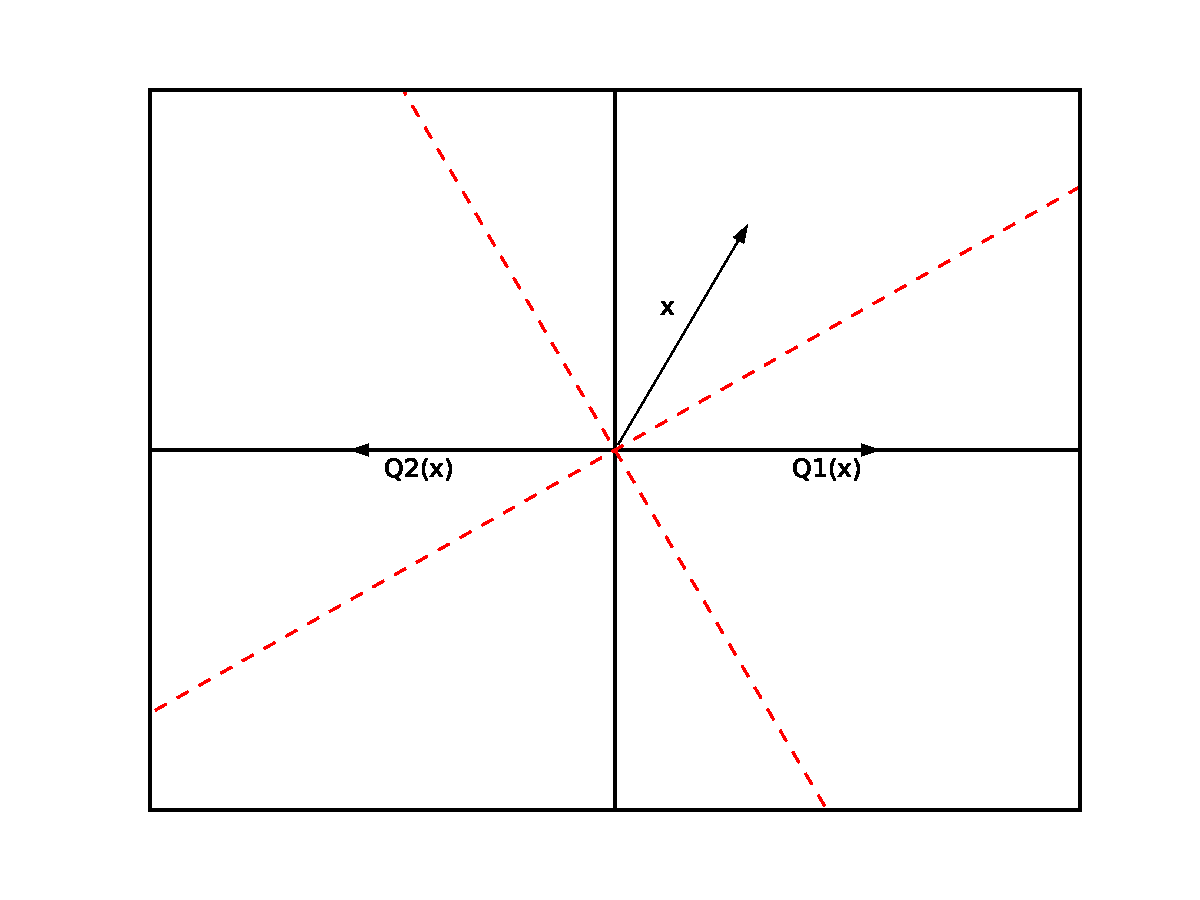
\includegraphics[width= \textwidth]{fig2}
	\caption{two reflectors}
	\label{fig:two reflectors}
\end{figure}

\begin{pseudo}{Householder triangularization}{A}
\label{Alg:Householder triangularization}
m,n \GETS size(A)\\
\FOR k \GETS 1 \TO n-1 \DO
\BEGIN
   x = A_{k:m,k}\\
   v_k = sign(x_1)\norm{x}_2 e_1 + x\\
   v_k = v_k / \norm{v_k}_2\\
   P_k = eye(m,m)\\
   P_k[k:m,k:m] = P_k[k:m,k:m] - 2 v v^T\\
   A = sp.dot(P_k,A);
\END
\end{pseudo}

This algorithm returns upper triangular $R$. You can find $Q$ s.t. $QR = A$ by multiplying the $P_k$ together appropriately.

\begin{problem}
\label{prob:HouseholderQR}
Write a script using Householder reflections to find the QR decomposition of a matrix A.
\end{problem}

\subsection*{Stability of the Householder QR algorithm}

Try the following in Python.

\begin{lstlisting}
In [1]:  import scipy as sp
In [2]:  import numpy.linalg as la
In [3]:  import my_householder
In [4]:  Q,X = la.qr(sp.rand(50,50)) #create a random orthogonal matrix:
In [5]:  R = sp.triu(sp.rand(50,50)) # create a random upper triangular matrix
In [6]:   A = sp.dot(Q,R) #Q and R are the exact QR decomposition of A
# use your Householder QR script to estimate Q and R:
In [7]:   Q1,R1 = my_householder.qr(A)
#now check the relative errors of Q1 and R1
In [8]:  la.norm(Q1-Q)/la.norm(Q)
Out [8]:  0.282842955725
In [9]:  la.norm(R1-R)/la.norm(R)
Out[9]:  0.0428922016647
\end{lstlisting}
This is terrible! Python works in $16$ decimal points of precision. But $Q_1$ and $R_1$ are only accurate to $0$ and $1$ decimal points, respectively. We've lost $16$ decimal points of precision!

Don't lose hope. Check how close the product $Q_1 R_1$ is to $A$.
\begin{lstlisting}
In [10]:  A1 = sp.dot(Q1,R1)
In [11]:  la.norm(A1-A)/la.norm(A)
Out[11]:  9.73996046986e-16
\end{lstlisting}
We've now recovered $15$ digits of accuracy. The errors in $Q_1$ and $R_1$ were somehow ``correlated," so that they canceled out in the product. The errors in $Q_1$ and $R_1$ are called \emph{forward errors}. The error in $A_1$ is the \emph{backward error}. The Householder $QR$ algorithm is a backward stable algorithm.

Householder QR factorization is more numerically stable than Gram-Schmidt or even Modified Gram-Schmidt (MGS). However, MGS is still useful for some types of iterative methods, because it finds the orthogonal basis one vector at a time instead of all at once (for example see Lab \ref{Ch:EigSolve}).

\subsection*{Upper Hessenberg Form}

%I'm not sure about this math. Is this true in the real case?
An upper Hessenberg matrix is a square matrix with zeros below the first subdiagonal. Every  $n \times n$ matrix $A$ can be written $A = Q^THQ$ where $Q$ is orthogonal and $H$ is an upper Hessenberg matrix, called the Hessenberg form of $A$. Note the similarity of this decomposition to the Schur decomposition in Lab \ref{Ch:Jordan}. 

The Hessenberg decomposition can be computed using Householder reflections, in a process very similar to Householder triangularization. Let's demonstrate this process on a $5 \times 5$ matrix $A$. Note that $A=Q^THQ$ is equivalent to $QAQ^T = H$; thus our strategy is to multiply $A$ on the right and left by a series of orthogonal matrices until it is in Hessenberg form. If we try the same $Q_1$ as in the first step of the Householder algorithm, then with $Q_1 A$ we introduce zeros in the first column of $A$. However, since we now have to multiply $Q_1 A$ on the left by $Q_1^T$, all those zeros are destroyed, as demonstrated below. (Although this process may seem futile now, it actually does tend to decrease the size of the subdiagonal entries. If we repeat it over and over again, the subdiagonal entries will often converge to zero. That's the idea behind the $QR$ algorithm in Lab \ref{Ch:EigSolve}.)
\[
\begin{array}{ccccc} 
\begin{pmatrix}
* & * & * & * & *\\
* & * & * & * & *\\
* & * & * & * & *\\
* & * & * & * & *\\
* & * & * & * & *\\
\end{pmatrix} 
&\underrightarrow{Q_1 \cdot }&
\begin{pmatrix}
* & * & * & * & *\\
0 & * & * & * & *\\
0 & * & * & * & *\\
0 & * & * & * & *\\
0 & * & * & * & *\\
\end{pmatrix} 
&\underrightarrow{\cdot Q_1^T }&
\begin{pmatrix}
* & * & * & * & *\\
* & * & * & * & *\\
* & * & * & * & *\\
* & * & * & * & *\\
* & * & * & * & *\\
\end{pmatrix} 
\\ 
A & & Q_1A & & Q_1 A Q_1^T
  \end{array}
\]
Instead, let's try starting with a different $Q_1$ that leaves the \emph{first} row alone and reflects the \emph{rest} of the rows into the range of $e_2$. This means that $Q_1^T$ leaves the first column alone.
\[
\begin{array}{ccccc} 
\begin{pmatrix}
* & * & * & * & *\\
* & * & * & * & *\\
* & * & * & * & *\\
* & * & * & * & *\\
* & * & * & * & *\\
\end{pmatrix} 
&\underrightarrow{Q_1 \cdot }&
\begin{pmatrix}
* & * & * & * & *\\
* & * & * & * & *\\
0 & * & * & * & *\\
0 & * & * & * & *\\
0 & * & * & * & *\\
\end{pmatrix} 
&\underrightarrow{\cdot Q_1^T }&
\begin{pmatrix}
* & * & * & * & *\\
* & * & * & * & *\\
0 & * & * & * & *\\
0 & * & * & * & *\\
0 & * & * & * & *\\
\end{pmatrix} 
\\ 
A & & Q_1A & & Q_1 A Q_1^T
  \end{array}
\]
We now iterate through the matrix until we obtain
\begin{equation*}
Q_3 Q_2 Q_1 A Q_1^T Q_2 ^T Q_3^T = 
\begin{pmatrix}
* & * & * & * & *\\
* & * & * & * & *\\
0 & * & * & * & *\\
0 & 0 & * & * & *\\
0 & 0 & 0 & * & *\\
\end{pmatrix} 
\end{equation*}

\begin{problem}
Write a script that transfers an input matrix to upper Hessenberg form. (Hint: You only need to modify your code code from problem \ref{prob:HouseholderQR} slightly.) We will use this technique in the eigenvalue lab later.
\end{problem}

\section*{Givens rotations}

The matrix $\begin{pmatrix} cos(\theta) & -sin(\theta) \\ sin(\theta) & cos(\theta) \end{pmatrix}$ rotates a vector counterclockwise by $\theta$. Given a vector $x = \begin{pmatrix} a \\ b \end{pmatrix}$, we can rotate $x$ into the range of $e_1$ by choosing the correct $\theta$. The problem is equivalent to solving for $c = cos(\theta)$ and $s = sin(\theta)$ in the system
\begin{equation}
\label{eq:Givens rotation system}
\begin{pmatrix} c & -s \\ s & c \end{pmatrix} \begin{pmatrix}a\\b\end{pmatrix} 
= \begin{pmatrix}r\\0\end{pmatrix}
\end{equation}
 In fact, it's not necessary to compute $\theta$; we solve for $c$ and $s$ directly. An obvious solution is $c = \frac{a}{\sqrt{a^2 + b^2}}$ and $s = \frac{b}{\sqrt{a^2+b^2}}$.

\subsection*{Givens triangularization}

Like Householder, the Givens $QR$ algorithm, \emph{triangularizes} a matrix $A$ using \emph{orthogonal transformations}. The Householder $QR$ algorithm worked one column at a time; Givens works one element at a time. Each nonzero below the main diagonal can be zeroed out with a Givens rotation. If we solve for $c$ and $s$ as above, the matrix
\begin{equation*}
G(i,j,c,s) = 
\begin{pmatrix}
1   & \cdots & 0 & \cdots & 0 & \cdots & 0 \\
 \vdots & \ddots & \vdots &  & \vdots & & \vdots \\
0   & \cdots &    c   & \cdots &    -s   & \cdots &    0   \\
 \vdots &        & \vdots & \ddots & \vdots &        & \vdots \\
 0   & \cdots &   s   & \cdots &    c   & \cdots &    0   \\
\vdots &        & \vdots &        & \vdots & \ddots & \vdots \\
0   & \cdots &    0   & \cdots &    0   & \cdots &    1 
\end{pmatrix}
\end{equation*}
where
\[ \begin{array}{ll}
g_{i\, i} = c  & g_{j\, i}= -s   \\
g_{j\, j} = c &  g_{i\, j}= s  \\
\end{array}\]
rotates by $\theta$ in the $i,j$ plane. Also, it's easy to check that $G(i,j,c,s)$ is orthogonal. Left-multiplying $A$ by $G(i,j,c,s)$ zeroes out $A_{i\, j}$. For example, 

\[
\begin{array}{ccccccc}
\begin{pmatrix}
*&*&*\\
*&*&*\\
*&*&*
\end{pmatrix}
&
\underrightarrow{G(3,1)}
&\begin{pmatrix}
*&*&*\\
*&*&*\\
0&*&*
\end{pmatrix}
&
\underrightarrow{G(2,1)}
&\begin{pmatrix}
*&*&*\\
0&*&*\\
0&*&*
\end{pmatrix}
&
\underrightarrow{G(3,2)}
&\begin{pmatrix}
*&*&*\\
0&*&*\\
0&0&*
\end{pmatrix}
\end{array}
\]

The Givens QR method is often slower than Householder, because it works one element at a time. But it is faster than Householder when $A$ is sparse, and it is very parallelizable.

\begin{problem}
Write a script that uses Givens rotations to do $QR$ decomposition. By performing successive Givens rotations, triangularize $A$ to find $R$. You can find $Q$ using the chain of rotations.

To find each rotation, you will have to solve \eqref{eq:Givens rotation system} for $c$ and $s$. Let $b$ be the element you want to zero out, say $A_{i\,j}$. Then $a$ is in the same \emph{column} as $b$, and in the \emph{row} you want to rotate into (it's like we're squishing the whole vector into $a$'s spot.) You can choose $a$ to be the diagonal element above $b$.
\end{problem}

\begin{problem} 
Compare the MGS, Householder, and Givens algorithms for $QR$ decomposition on various matrices. Try different sizes and different levels of sparsity. Which is the fastest? Which is the most stable?
\end{problem}


%Sources: http://www.cs.unc.edu/~krishnas/eigen/node5.html
% http://en.wikipedia.org/wiki/Givens_rotation
%http://en.wikipedia.org/wiki/QR_decomposition
%	Note the Operation count: Householder is 2/3 n^3, MGS is 2 n^3
%http://en.wikipedia.org/wiki/QR_algorithm
%Applied Numerical methods using MATLAB by Yang has some code written for this
%http://www.math.kent.edu/~reichel/courses/intr.num.comp.2/lecture21/evmeth.pdf
%	These are eigenvalue algorithms explained carefully
%http://en.wikipedia.org/wiki/Householder_transformation
%Numerical Linear Algebra, by Lloyd N. Trefethen and David Bau III, Chapters 10 and 16